\newpage
\section{Моделирование}

\subsection{Математическое моделирование}

\subsubsection{Модель ``Hybrid Stepper Motor'' из пакета ``SimPower Systems''}

Для моделирования процессов, протекающих в системе, воспользуемся пакетом MATLAB.
Перед построением модели всей системы, необходимо получить все параметры,
необходимые для использования встроенной модели гибридного шагового двигателя из пакета:

\textit{SimPower Systems -> Second Generation -> Motors and Generators -> Hybrid Stepper Motor.}

Известно всё необходимое, за исключением величины потосцепления, формируемого
постоянными магнитами ротора. Его можно определить по формуле
из \cite{Matlab_help_stepper_motor}:

\begin{equation}
    \label{maximum_flux_linkage}
    \psi_{M} = \frac{30}{\pi p} E_{M} N
\end{equation}

$N$ - частота вращения ротора, об/мин

$$
    p = \frac{360}{2m \cdot step}
$$

$m = 2$ - число фаз шагового двигателя

$step = 1,8$ - шаг углового перемещения шагового двигателя, град

$E_{M}$ - амплитудное значение ЭДС самоиндукции разомнутой обмотки статора, В

Для использования (\ref{maximum_flux_linkage}) проведём следующий эксперимент:
с помощью дополнительного двигателя на стенде разгоним интересующий нас шаговый
двигатель до частоты вращения $N = const$ и с помощью осцилографа определим $E_{M}$
в одной из его разомкнутых обмоток.

\subsubsection{Модель в ``MATLAB Simulink''}
Обозначим процессы, модерируемые в работе привода на созданной модели:

\begin{itemize}
    \item Токовые контуры в обмотках двигателя
    \item Сухое и вязкое трение
    \item 3 среднечастотных резонансных гармоники (см. \ref{Novel_Modeling_and_Damping})
\end{itemize}

В созданной модели используется следующие допущения:

\begin{itemize}
    \item Пусть момент двигателя пропорционален току, то есть пренебрежем той частью переходных
            процессов, где это не так
\end{itemize}

\paragraph{ Токовые процессы }
Для контура одной фазы двигателя, пренебрегая наличием ёмкости внутри обмоток, можно записать
закон Ома:

Для фазы A:
\begin{equation}
    \frac{di_{a}}{dt} =
        - \frac{R}{L_{0}} i_{a}
        + \frac{K_{T}}{L_{0}} \omega_{r} \sin(N_{r}\theta)
        + \frac{\vartheta_{A+} - \vartheta_{A-}}{L_{0}}
\end{equation}

Для фазы B:
\begin{equation}
    \frac{di_{b}}{dt} =
        - \frac{R}{L_{0}} i_{b}
        - \frac{K_{T}}{L_{0}} \omega_{r} \cos(N_{r}\theta)
        + \frac{\vartheta_{B+} - \vartheta_{B-}}{L_{0}}
\end{equation}
%% здесь надо вставить рисунок кусока модели реализующей эти уравнения
\begin{figure}[ht!]
    \centering
    \includegraphics[width=0.8\textwidth, keepaspectratio]
                    {./src/pictures/drive_model/drive_model_current_equation}
    \caption{Реализация физики электрических процессов фазы шагового двигателя в модели}
    \label{pic_drive_model_current_equation}
\end{figure}

\paragraph{ Уравнения для момента }
Будем считать, что момент пропорционален току в некотором рабочем диапазоне. Тогда можно записать:
$$
    \tau_{a} = - K_{T} i_{a} \sin{N_{r} \theta}
$$
$$
    \tau_{b} = K_{T} i_{b} \cos{N_{r} \theta}
$$
Запишем суммарный момент как сумму двух вышеописанных составляющих:
\begin{equation}
    \tau = K_{T} [-i_{a} \sin{N_{r}\theta} + i_{b} \cos{N_{r}\theta}]
\end{equation}

%% здесь надо вставить рисунок куска модели, реализующей эти уравнения

\paragraph{ Диссипативные силы }
В модели учитывается 2 составляющие трения - вязкое и сухое.

Вязкое трение аппроксимировано до составляющей, пропорциональной первой производной от угла поворота:
\begin{equation}
    \tau_{\text{тр.вязк.}} = D_{f} \omega_{r}
\end{equation}

Сухое трение получено из формулы:
\begin{equation}
    \tau_{\text{тр.сух.}} = \begin{cases}
         |\tau| \cdot \frac{\omega_{r}}{|\omega_{r}|}, & \text{если} ~|\tau|  <  D_{d}; \\[2mm]
         D_{d}  \cdot \frac{\omega_{r}}{|\omega_{r}|}, & \text{если} ~|\tau| \ge D_{d}.
    \end{cases}
\end{equation}

\begin{equation}
    \tau_{\text{тр.}} = \tau_{\text{тр.вязк.}} + \tau_{\text{тр.сух.}}
\end{equation}

\begin{figure}[ht!]
    \centering
    \includegraphics[width=0.7\textwidth, keepaspectratio, clip=true, trim=25mm 35mm 25mm 35mm]
                    {./src/pictures/drive_model/drive_model_friction}
    \caption{Реализация диссипативных сил в модели}
    \label{pic_drive_model_friction}
\end{figure}

%% здесь надо вставить рисунок куска модели, реализующей эти уравнения

\paragraph{ Среднечастотная нестабильность }
Согласно \cite[ф-ла 5]{Novel_Modeling_and_Damping}, можно выделить три основных
гармоники среднечастотной нестабильности \[1, 2, 4\].
\begin{equation}
    \tau_{\text{рез.}} =   K_{d1} \cdot \sin{ (  N_{r} \theta + \phi_{1}) }
                         + K_{d2} \cdot \sin{ (2 N_{r} \theta + \phi_{2}) }
                         + K_{d4} \cdot \sin{ (4 N_{r} \theta + \phi_{4}) }
\end{equation}

$K_{d1}$ - амплитуда первой гармоники резонанса момента

$K_{d2}$ - амплитуда второй гармоники резонанса момента

$K_{d4}$ - амплитуда четвертой гармоники резонанса момента

$\phi_{1}$ - фаза первой гармоники резонанса момента

$\phi_{2}$ - фаза второй гармоники резонанса момента

$\phi_{4}$ - фаза четвертой гармоники резонанса момента

Третья, пятая и более высокие гармоники оказывают незначительное влияние, а потому
ими можно и нужно пренебречь.
%% здесь надо вставить рисунок куска модели, реализующей эти уравнения

\newpage
\subsection{Натурное моделирование}
Разработка стенда для валидации математической модели, изучения влияния внешний параметров
на качество работы алгоритмов управления, изучение резонанстных явлений в шагвом
двигателе планируется в ближайшее время.

Осюда можно сформулировать требования к разрабатываемой модели.
\begin{itemize}
    \item Модель должна содержать в себе полноценный двигатель из разрабатываемого
    привода для моделирования физических процессов в электрических и магнитных цепях.

    \item Должна быть имитация полной нагрузки с моментом инерции не менее чем
    значение указанное в техническом задании, в том числе для того, что бы оценить
    грузоподъемность разрабатываемого привода, его быстродействия на максимальных
    нагрузках, а так же, что не менее важно, позволит с некоторой точностью
    определить положенияе на частотной оси резонанстных явлений.

    \item Обязательно, должно быть устройство имитации сухого трения. Как
    известно сухое трение может оказывать отрицательное влияние на устойчивость
    и точность системы.

    \item В механической связи между двигателем и нагрузкой? должна быть имитация
    упругости редуктора привода, так как, это может иметь отрицательный эффект
    для точности конечного механизма.

    \item В модели должен стоять один или более датчиков угла, с точностью не
    грубее чем датчик который планируется установить на привод. В идеале должно
    стоять двадатчика: точный для экспериментальных целей и грубый близкий
    к тому что предполагается поставить на привод манипулятора.

    \item Стенд должен обеспечивать легкий доступ к электрическим цепям двигателя,
    усилителя тока и микропроцессорного блока управления для снятия сигналов
    осцилографом.

    \item Конструкция должна иметь массивное основание, ровно настолько чтобы
    исключить вероятность опрокидывания конструкции при реверсивных движениях
    и переброске на максимальном ускорении.

    \item Статическа конструкция в нормальных условаия работы по техническому
    заданию отстутствует, и по этой причине в модели ее учитывать не нужно.
\end{itemize}

\endinput

